% This file is part of the `speccal` project.
% Copyright 2014 the authors.
% All rights reserved.

% ## style notes:
% - all equations in `eqnarray` environments
% - use `\,` as the multiply operator!
% - parameters are `inferred`; `measurement` is reserved for data
% - use emulateapj or aastex, as you like, but watch for equation-wrapping in the former

% ---- Hogg (aastex) mode ----
%\documentclass[12pt, letterpaper, preprint]{aastex}
% ----


% ---- Charlie (emulateapj) mode ----
 \documentclass[iop,numberedappendix]{emulateapj}
 \usepackage{apjfonts}
% ----
\usepackage{color, hyperref}
\bibliographystyle{apj}
%\input{vc}

% math shih
\newcommand{\transpose}[1]{{#1}^{\!\mathsf T}}
\newcommand{\given}{\,|\,}
\renewcommand{\det}[1]{||{#1}||}

% affiliation marks; edit with care
\newcommand{\lick}{1}
\newcommand{\ccpp}{2}
\newcommand{\cds}{3}
\newcommand{\mpia}{4}

%figures
\usepackage{graphicx}
\DeclareGraphicsExtensions{.png,.pdf}
\newcommand{\excluster}{NGC7089}

%references
\newcommand{\foreign}[1]{\emph{#1}}
\newcommand{\etal}{\foreign{et\,al.}}


\begin{document}\sloppy\sloppypar
\title{Combining information from photometric and spectroscopic data:\\
  propogating uncertainties in spectrophotometric calibration}
\shorttitle{Combining Spectroscopy and Photometry}
\author{
  BDJ\altaffilmark{\lick},
  DRW\altaffilmark{\lick},
  DFM\altaffilmark{\ccpp},
  DWH\altaffilmark{\ccpp, \cds, \mpia},
  CC\altaffilmark{\lick},
  others}
\shortauthors{bdj et al}
\altaffiltext{\lick}{University of California Lick Observatory}
\altaffiltext{\ccpp}{Center for Cosmology and Particle Physics, Department of Physics, New York University}
\altaffiltext{\cds}{Center for Data Science, New York University}
\altaffiltext{\mpia}{Max-Planck-Institut f\"ur Astronomie}

\begin{abstract}
In a typical spectral-fitting project,
  there tend to be a small number of bands of well-calibrated photometry
  and thousands of poorly calibrated spectroscopic pixels.
Good spectroscopic calibration is both expensive and difficult,
  but naive weighted least-square fitting will weight
  the thousands of spectroscopic pixels far higher overall
  than the few photometric bands.
Here we present a flexible and general spectroscopic calibration model,
  which can be fit simultaneously along with whatever spectral parameters.
The model involves a polynomial calibration vector to capture large-scale calibration issues
  and a Gaussian Process to capture small-scale wiggles.
We show that, in this framework, the quality of some kinds of spectral parameter fits
  is not a strong function of the quality of the spectroscopic calibration;
  that is, for many scientific goals there is no scientific reason
  to obtain good---or really any---spectrophotometric calibration.
In particular, for stellar population fitting, high signal-to-noise data,
  and good photometry,
  we show that raw counts are just as good as calibrated counts for making inferences about the
  parameters of interest.
This obviation of calibration overheads will pay \emph{all yall mad cheddar},
  at least if yall employ full cost accounting.
\end{abstract}

\keywords{
  greetings
  ---
  whole world
}

\section{Introduction}

In probabilistic inference, all information flows from the data to the
parameters of interest by means of a likelihood function, or an
expression for the probability of the data conditioned on the
parameters.
If there are $N$ independent sources of data, for each of which there
is a likelihood function, the full-data likelihood is the product of
the $N$ individual likelihoods (or the log-likelihood is a sum of the
$N$ individual log-likelihoods).
There is no bespoke ``weighting'' of the data that is justifiable in
this framework.
This creates some apparent paradoxes!
One is the following:

Imagine you have three photometric bands through which you have
observed some object (independently, say), and also a 2500-pixel
spectrum, where the pixels are defined such that they are precisely or
approximately independent measurements.
For these purposes, two spectral pixels are very close to independent
measurements if they are derived from disjoint sets of detector pixels
in the spectrograph detector plane.
Each photometric band and each spectroscopic pixel has a
log-likelihood function, and these 2503 log-likelihood functions must
be (by the Rules of Righteousness) coadded equally into one full-data
log-likelihood.
The log-likelihood is therefore fully dominated by the spectral
pixels!
This despite the fact that in almost all astronomical investigations,
the photometry is far more reliable, per measurement, than the
spectra.
That is, if the spectral pixels tend to prefer one model, or one set
of parameters, and the photometry another, the spectra will almost
always ``win'' just by their overwhelming numbers.

What is a Righteous Probabilistic Investigator (RPI) to do?
One option---fully unjustified---is to ``down-weight'' the
log-likelihoods of the spectral pixels relative to the photometric
measurements.
This is equivalent to taking the likelihoods to some power, which has
no justification in inference (though it is sometimes used in
optimization and sampling as an ``annealing'' move).
This down-weighting is not justified, but there is even more
ad-hockery than this, because there is no principled way to choose the
unprincipled weights.

The Right Thing To Do is to express the \emph{reason} that the RPI
believes the spectroscopic data to be less reliable \emph{within} the
likelihood function.
That is, the RPI must add nuisance parameters to parameterize the
unreliability of the spectroscopy, and infer those along with the
parameters of interest.
If this parameterization is good, the information in the spectroscopy
data will not flow entirely to the parameters of interest; instead,
some will flow to the nuisance parameters.
This will reduce the importance of the spectroscopy relative to the
photometry and the RPI will be well pleased with the dominance of the
photometric data in the final inferences of the parameters of
interest.
This amounts to propogating the uncertainties in the
spectrophotometric calibration (or alternatively in the continuum
normalization).
In what follows, we provide an example of this kind of
parameterization and inference.

Our example involves instantiating a ``calibration adjustment'' model,
which itself has both a polynomial component and a non-parametric
component.
The parameters of the calibration adjustment are nuisances, from a
scientific standpoint.
However, because the calibration adjustment is inferred along with the
parameters of interest, the probabilistic inference that provides
parameter estimates \emph{also} provides a spectrophotometric
calibration of the spectral data.
That is, the method we present has the potential to \emph{obviate
spectrophotometric calibration}.

We find that this potential---obviation of calibration---is realized.
That is, if the procedures demonstrated below become widely adopted,
some or perhaps most astronomical spectroscopic projects could
potentially drop or dramatically reduce their spectrophotometric
calibration programs.
This would reduce telescope overheads and data-analysis time and
complexity, delivering economic and sanity benefits to the whole
community.

\section{Model generalities}

THIS SECTION NEEDS WORK; THIS IS JUST AN EQUATION DUMP.

HOGG: A model is a parameterized likelihood function, with prior PDFs on the nuisance parameters (at least)...

HOGG: There is a likelihood for the photometry and for the spectroscopy...

HOGG: Each of these penalizes the difference between a column vector of data and a column vector of model expectation value...

The standard chi-squared or log-Gaussian log-likelihood is
\begin{eqnarray}
\ln p(d\given\theta) &=& -\frac{1}{2}\,\sum_{n=1}^N \left[\frac{[d_n - \mu_n(\theta)]^2}{\sigma_n^2} + \ln(2\pi\,\sigma_n^2) \right]
\quad ,
\end{eqnarray}
where $\theta$ is a blob of parameters of interest,
$d$ is the full set (in the form of a column vector) of data,
made up of $N$ values $d_n$,
$\mu(\theta)$ is the the column-vector mean prediction (expectation value) of the model,
made up of $N$ values $\mu_n(\theta)$,
the $\sigma_n^2$ are the observational noise variances.
We have included the $\ln(\sigma_n^2)$ term in the likelihood because
in what follows we are going to be modifying the noise model.

If you don't believe the reported data noise variances $\sigma_n^2$,
it often makes sense to add in quadrature a ``jitter'' variance
$s^2$.  For photometric data this ``jitter'' is often best described
as a fractional error, $(\hat{s}\mu(\theta))^2$, corresponding for example
to an additional magnitude zero-point uncertainty.
This is a simple modification of the chi-squared log-likelihood:
\begin{eqnarray}\label{eq:photometricLF}
\ln p(d\given\theta,s^2) &=& -\frac{1}{2}\,\sum_{n=1}^N
                             \left[\frac{[d_n - \mu_n(\theta)]^2}
                             {[\sigma_n^2 + s^2]} + 
                             \ln(2\pi\,[\sigma_n^2 + s^2]) \right]
\quad .
\end{eqnarray}
This modification shows the necessity of including the log-variance
term.
This---equation~(\ref{eq:photometricLF})---is in fact the
log-likelihood function we are going to use for the photometric
measurements in what follows.  In this formulation, if $\theta$ are
the parameters of interest, the jitter variance $\hat{s}^2\equiv
s/\mu(\theta)$ is a nuisance noise-model parameter representing
additonal fractional uncertainty in the flux.  The Gaussian Process
will be a generalization of this modification.

We take the calibration-vector that modifies the mean model to produce
the observed spectrum as multiplicative with respect to the mean
model.  In this case we define the residual of the data from the model
in terms of the logarithmic differences.  This logarithmic formulation
requires that $d$ be everywhere positive, and distorts the
uncertainties, especially at low S/N ratio.  The advantages of
defining the residual in this way are that the model remains linear
(and therefore fast) and the calibration vector is forced to be
positive everywhere.  Additionally, at high signal to noise the
distortion of the uncertainties will be minimal.

The calibration-vector and Gaussian-Process modified log-likelihood is
\begin{eqnarray}\label{eq:spectroscopicLF}
\ln p(d\given\theta,\alpha) &=& -\frac{1}{2}\,\left[\transpose{\Delta}\,C^{-1}\,\Delta + \ln([2\pi]^N\,\det{C}) \right]
\\
\Delta &\equiv& \ln d - \ln \mu(\theta) - f(\alpha) 
\\
C_{nn'} &\equiv& [\hat{\sigma}_n^2 + s^2]\,\delta_{nn'} +
K_\alpha(\lambda_n - \lambda_{n'})
\\
\hat{\sigma_n} & = &\sigma_n/d
\quad ,
\end{eqnarray}
where $\alpha$ is a blob of nuisance parameters
(which determine the jitter, the calibration vector and the kernel function),
$\Delta$ is a residual column vector,
$f(\alpha)$ is a calibration column vector,
$C$ is the Gaussian Process covariance matrix,
made up of $N^2$ values $C_{nn'}$,
$K_\alpha$ is a kernel function that sets the wavelength scale and
amplitude of the residual calibration issues,
$\hat{\sigma}_n$ are the fractional uncertainties of the data,
and each $\lambda_n$ is the wavelength of spectral pixel $n$.
The calibration vector $f(\alpha)$ is going to take care of the
large-scale calibration residual; the Gaussian Process is going to
pick up smaller-scale residuals away from \emph{that}.
The flexibility of the Gaussian Process specified by $C$ will obviate
the need for numerous high order polynomial terms in $f(\alpha)$ and
thus reduce the number of free parameters required in the model.  The
prior over functions implied by $C$ is analytically conditioned on the
residuals $\Delta$.
The residual column vector is defined in terms of the logarithmic
difference between the data and the mean model $\mu$ since we are
taking the calibration vector to be multiplicative with respect to
the mean model $\mu$. In this formulation the the mean model $\mu$ will be effectively
multiplied by $e ^{f(\alpha)}$ 
This---equation~(\ref{eq:spectroscopicLF})---is the log-likelihood we
are going to use for the spectroscopic data in what follows.

In detail, we are going to choose a $M$th-order polynomial form for
the calibration vector $f(\alpha)$ and a bell shape (Gaussian) for the
kernel function $K_\alpha(\cdot)$:
\begin{eqnarray}\displaystyle
f(\alpha) &=& c_0\,[1 + \sum_{m=1}^M c_m\,x^m]
\\
x &\equiv& \frac{\lambda}{\lambda_0} - 1
\\
K_\alpha(\lambda_n - \lambda_{n'}) &=& a^2\,\exp(-\frac{[\lambda_n - \lambda_{n'}]^2}{2\,\ell^2})
\\
\transpose{\alpha} &\equiv& \left[ \{c_m\}_{m=0}^M, s^2, a^2, \ell^2 \right]
\quad ,
\end{eqnarray}
where $\lambda$ is a column vector made up of the wavelengths $\lambda_m$
and $x$ is a scaled and shifted version of the same,
scaled by a fiducial wavelength $\lambda_0$.
Nuisance parameters $c_m$ set the shape of the large-scale calibration
issues, while $a^2$ and $\ell^2$ set the variance and correlation
length of the remaining covariant calibration noise.


XXX Alternative XXX
To avoid making the logarithmic transform described above, which
distorts the errors, we can formulate the problem in a different way,
modifying Equation \label{eq:spectroscopicLF} above as 
\begin{eqnarray}\label{eq:spectroscopicLF_v2}
\ln p(d\given\theta,\alpha) &=&
                                -\frac{1}{2}\,\left[\transpose{\Delta}\,C^{-1}\,\Delta
                                + \ln([2\pi]^N\,\det{C}) \right]
\\
\Delta &\equiv& d - \mu(\theta) * f(\alpha) 
\\
C_{nn'} &\equiv& [\sigma_n^2 + (\hat{s} * \mu)^2]\,\delta_{nn'} +
\transpose{\mu} \, K_\alpha(\lambda_n - \lambda_{n'}) \, \mu
\quad ,
\end{eqnarray}
where the multiplication of $s$ and $K_\alpha$ by $\mu$ in the
construction of $C_{nn'}$ means that they are defined in
\emph{fractional} terms, and the uncertainties remain Gaussian in
linear flux space.  It remains to be seen whether this actually works.



\section{Data and Experiments}

We are now left to demonstrate that, by including photometry as well
as spectroscopy, it is possible to infer the parameters of interest
$\theta$ while marginalizing over the calibration parameters $\alpha$.
We will apply the methodology for spectrophotometric calibration
described above to both \emph{mock} and \emph{real} optical spectra of
Galactic globular clusters.  Spectra of globular clusters provide a good test case,
as they are less complex than galaxy spectra (for which it is
necessary to model the star formation history) but are by no means
trivial. In this way the key features of the calibration model and
methodology are not obscured.  Additionally, information
about the physical parameters of the cluster is available from
resolved stellar CMDs, providing an important check on our inference methodology
and especially our population synthesis models.

This separate treatment of mock and real data allows us to address two
separate issues.  The inference from mock data (with a realistic
calibration vector applied) provides a test of the methodology and the
effect of calibration uncertainties on the inferred parameters in the
case of a perfect mean model $\mu(\theta)$.  The inference from real
data tests a combination of our methodology and the ability of the
population synthesis models to recover parameters inferred from
resolved star CMDs (i.e. some estimate of ground truth).

To demonstrate the effectiveness of our strategy for combining
spectroscopic and photometric information we will infer the parameters
$\theta$ from a spectrum both \emph{before} and \emph{after} it has
been spectrophotometrically calibrated using and
ancillary spectrophotometric calibration data.



\subsection{Real Data}

The data we use to test our method consist of optical spectroscopy of
of galactic globular clusters from \citet{schiavon05} for which
optical and NIR photometry are available. The optical spectra were
obtained by drift-scanning a long-slit spectrograph across the
cluster.  The wavelength range of the spectra is $3500-6500$\AA. The
instrumental resolution is $\sim 3.1$\AA~ at $\sim 4500\AA$ and varies
with wavelength.  These spectra have been placed on the rest-frame,
though in what follows we will model the effect of redshift
uncertainties on the data.

An example spectrum (and the inferred spectrophotometric calibration
vector) is shown in Figure \ref{fig:ggc_data}.  As stated by
\citet{schiavon05}, the spectrophotometric calibration of these data are
only approximate.  When fitting the spectra we mask the region around
the bright OI5577\AA~ sky line, and we fit only to the spectrum with $3550\AA
< \lambda < 6500$\AA~ which are covered by the MILES spectral library
(see \S\ref{sec:cluster_model}).  Absorption lines of the interstellar
medium (ISM) can significantly affect the spectrum, so we
additionally mask the Calcium H and K lines and the NaD doublet.

Words about photometry.

\begin{table}[h!]
\caption{List all the clusters, RA, Dec, photometry and individual exposures.}
\end{table}


\subsection{Mock Data}
Our mock data are designed to mimic the actual data as much as
possible.  Mock spectra and photometry are generated from the model
described in below (\S\ref{sec:cluster_model}, equation
\ref{eq:MeanModel}) for a given set of parameters $\theta^\prime$.  We
then convolve the spectrum with an instrumenal LSF, interpolate onto
the observed wavelength scale and add noise according to the SNR of
the real data.  For the photometry we assume a SNR of 10.  We also
mask the mock spectra at the location of significant sky lines and ISM
lines that are present in the real data.

We will refer to these spectra as the \emph{perfectly calibrated} mock
spectrum.  An example is shown in Figure \ref{fig: mock data}. We also
produce mock spectra by dividing the perfectly calibrated spectra by
the spectrophotometric calibration vector taken from the real data
\citep[][Fig\ref{fig:ggc_spectrum}]{schiavon05}.  We refer to these as
the \emph{uncalibrated} mock spectra.

\subsection{Star Cluster Model}
\label{sec:cluster_model}
We model the stellar cluster as a single age SSP. The spectrum of a
star cluster under this assumption is given by
\begin{eqnarray}\displaystyle
F_{\theta^\prime}(\lambda_o) & = &
\frac{m_*}{4\pi d_L^2(1+z)} \, S(\lambda, t, Z , \beta) \, e^ {-k_\lambda\tau_V} \\
\nonumber \\ 
\lambda_o & = & (1+z)\,\lambda 
\\
\theta^\prime & \equiv & \left[ m_*, t, Z, \tau_V, z, d_L, \beta \right]
\quad ,
\end{eqnarray} where the
parameters $\theta^\prime$ include 
the stellar mass $m_*$, 
effective optical depth to dust in the $V$-band $\tau_V$, 
luminosity distance $d_L$,
and redshift $z$.
The shape of the dust attenuation curve is given by $k_\lambda \equiv
\tau_\lambda/\tau_V$.  
The observed frame wavelengths $\lambda_o$ are related to the
restframe wavelengths $\lambda$ in the usual way.

The spectrum of one solar mass of stars that formed at lookback time
$t$ with metallicity $Z$ is given by $S(\lambda, t, Z [, \beta])$.
Here the additional parameters $\beta$ may include details of the
population synthesis model, such as the IMF slope and adjustments to
the stellar spectra or stellar evolutionary tracks. We will assume
$\beta$ to be fixed for the purposes of this exercise, with no loss of
generality but significant savings in computational time.  We will
also fix the shape of the attenuation curve, $k_\lambda $, to the
Milky way average of \citet{CCM89} with $R_V=3.1$ and assume that
$d_L$ is known to high precision from independent methods and can
therefore be treated as fixed.  In practice, $d_L$ is perfectly
degenerate with $m_*$. We calculate $S(\lambda, t, Z)$ using the
Flexible Stellar Population Synthesis code \citep[FSPS][]{fsps}.  We
use the Padova 2007 isochrones \citep{girardi00, bertilli94, marigo07}
and the MILES stellar spectral library \citep{miles_I, miles_II,
miles_III}.

Nebular emission lines (which may arise from HII regions around the
clusters or from diffuse ionized gas) and interstellar absorption
lines are modeled as a sum of Gaussians of unknown amplitude $A_\ell$,
all of the same width $\sigma_e$ (which need not be the same as
stellar broadening $\sigma$) and with known central wavelengths
$\lambda_\ell$.  For emission lines the amplitudes are constrained to
be positive, while for interstellar absorption (e.g. Na D and Ca K)
the amplitudes are constrained to be negative. This framework can be
easily extended to include more complex models for the nebular
emission, such as allowing line dependent widths and velocities, and
using Voight profiles for the line shapes.  

The model spectra $F_{\theta^\prime}$ are smoothed by convolution with
the line-spread function of the spectrograph and are interpolated to
the wavelength points of the of the observed spectrum while taking
into account the redshift. For computational simplicity we assume that
the internal velocity dispersion of the cluster is negligible compared
to the instrumental broadening, though in principle it can and should
also be modeled. The instrumental resolution is given by the parameter
$\sigma$.  {\color{blue}Discuss intrinsic resolution of model spectra
(MILES), what to do in situations where instrumental resolution is
higher, lower or comparable (ouch) to intrinsic velocity broadening.}


The final mean model is then given by the convolution in wavelength
\begin{eqnarray}\label{eq:MeanModel} 
\mu(\theta) &  = & (LSF(\sigma_{inst}) \otimes F(\theta^\prime))(\lambda) +
\sum_{\ell=0}^{N_\ell} S_\ell(\lambda) \\
S_\ell (\lambda) & = & \frac{A_\ell}{\sigma_e\sqrt{2\pi}} \exp(-\frac{(\lambda -
\lambda_\ell)^2}{2\sigma_e^2}) \\
\theta & \equiv & \left[ \{\theta^\prime\}, \sigma_{inst}, \{A_\ell\}_{\ell=0}^{N_l},
  \sigma_e \right] \\
\quad ,
\end{eqnarray}
where $LSF(\sigma_{inst})$ represents the linespread function
parameterized by $\sigma_{inst}$, 
$\otimes$ indicates convolution, 
and the full parameter set $\theta$ now includes
the instrumental broadening $\sigma_{inst}$ 
and the dispersion $\sigma_e$ and
amplitudes $A_\ell$ of the $N_l$ nebular emission and interstellar
absorption lines.
This is the mean model which appears in equation
\ref{eq:spectroscopicLF}.

To model the photometry we simply project the observed frame mean
model spectrum (equation \ref{eq:MeanModel}) onto the filters of
interest.  Note that we do \emph{not} include the calibration vector
$f(\alpha)$ in this projection.


\subsection{Sampling and Priors}

We estimate the posterior through MCMC sampling after an initial round
of optimization using Powell's method.  The specific sampling
algorithm we use is the affine-invariant ensemble sampling scheme of
\citet{goodman}, as implemented in the \texttt{emcee} package \citep{emcee}
Unlike typical Metropolis-Hastings MCMC sampling, the affine-invariant
sampler does not require the specification of step sizes in each
dimension.  {\color{blue}ASSESSING SAMPLER CONVERGENCE}
 
At each iteration of the sampler the photometric and spectroscopic
likelihood are computed, multiplied together, and multiplied by the
the prior probability of that parameter position to obtain an estimate
of the posterior probability for those parameters given the data.

Our prior distributions are in all cases top-hat functions, described
in Table \ref{tbl:priors}, though more informative prior distributions
may be used.  Informative priors may be especially appropriate for the
calibration parameters $\alpha$ if additional information about the
instrument is available; or for the parameters of interest $\theta$,
for example if there is knowledge of the metallicity
distribution of the population from which a given cluster is drawn.

\input{tables/priors.tbl}


\subsection{List of Experiments}

\begin{enumerate}

\item Mock perfectly calibrated data: inference using spectroscopy and one
  photometric band, with both full calibration model and assuming no
  calibration uncertainty.

\item Mock uncalibrated data:  inference using spectroscopy and one
  photometric band, with full calibration model 

\item Mock data: inference using photometry only

\item Mock uncalibrated data: inference using spectroscopy and all
  photometry, full calibration model.

\item Do this for a bunch of ages, metallicities, and dust
  attenuations, possibly compare to the ideal posteriors.

\item Real calibrated spectrum:   Inference using spectroscopy and all
  photometry, with full calibration model. 

\item Real uncalibrated spectrum:   Inference using spectroscopy and all
  photometry, with full calibration model. 

\item Compare the physical parameters inferred from from the real
  calibrated and uncalibrated spectrum with each other and with CMD
  based parameters.

\end{enumerate}

\section{Results}

For each test we want to show
\begin{itemize}

\item Posterior parameter pdfs (and joint pdfs).

\item Samples of the posterior prediction for the observations, and
  residuals thereform.

\item The calibration vector, and posterior samples of it.

\item Posterior samples of the intrinsic spectrum
\end{itemize}

\subsection{Mocks}
We first present the results of our inference from a spectrum where we
assume the calibration is known perfectly.  That is, we fix the
calibration parameters $\alpha$ to the values used to construct the
mock data.  This sets a baseline for the kind of posterior PDFs that
could be obtained for the physical parameters given the
signal-to-noise of the mock data, perfect models, and perfectly known
calibration.

{\color{blue}BDJ Describe results from the ideal case.}

Next we will \emph{not} assume that the calibration is perfectly known
and we will therefore allow the calibration parameters $\alpha$ in our
model to vary.  In Figure
\ref{fig:speconly_calibrated} we show the result of our inference from
the spectrum and a single photometric measurement (SDSS $g$) for a
perfectly calibrated mock spectrum. To demonstrate the quality of the
fit we show both the mock input spectrum and predictions of the
observed spectra that result from several draws of the model
parameters $[\theta, \alpha]$ from posterior distribution.  We also
show samples of the inferred calibration vector,
\begin{eqnarray} 
\frac{d}{\mu(\theta)} & = & e^{f(\alpha) + \tilde{\Delta}}
\quad ,
\end{eqnarray}
where $\tilde{\Delta}$ is the Gaussian Process mean prediction for the
logarithmic residual between the data and the model.  For the
perfectly calibrated spectrum the true calibration vector (shown in
black) is one everywhere.  The spread of the inferred calibration
vectors approximately indicates our uncertainty in the spectrophotometric
calibration when no additional calibration information is available
and only a single photometric point is available.


Even in the case of a single photometric data point, many of the
physical parameters are well-constrained and only minimally biased,
e.g. age and metallicity.  These are the parameters that are
constrained well by the spectrum itself and are not strongly sensitive
to the overall shape of the spectral continuum.  Such parameters can
be reasonably well recovered by fitting continuum normalized spectra,
though here we have propogated the uncertainty in this normalization
into the uncertainties on the physical parameters.

On the other hand, the posterior PDF for the dust attenuation optical
depth $A_v$ is extremely broad. 

The uncertainty on the total stellar mass incorporates both the
uncertainty in the photometric flux and the uncertainty in the $g$-
band mass-to-light ratio.

In Figure \ref{fig:speconly_uncalibrated} we show the results of
inference on an \emph{uncalibrated} mock spectrum.


\subsection{Real Data: NGCXXXX} 
We first infer the parameters of interest $\theta$ for a calibrated
spectrum of one of the clusters, \excluster, using the full YY-band
photometry. In Figure \ref{fig:inferred_spectrum} we show the spectra
that result from draws of the parameters $[\theta,\alpha]$ from the
posterior distribution, as well as several of the individual
components of the model constructed from each draw. Figure
\ref{fig:inferred_spectrum} also shows the calibrated spectrum on
which the priors were conditioned, and residuals between the posterior
models and the observed data.  

In Figure \ref{fig:inferred_sed} we show the corresponding SED for the
posterior parameter draws, compared to the observed SED. There is some
tension between the modeled and observed SEDs, I'm not quite sure
why. Finally, In Figure \ref{fig:inferred_params} we show the
marginalized and joint PDFs for a subset of the full model parameters.

It is possible to reconstruct the inferred total multiplicative
calibration vector for each draw of the model parameters.  Rearranging
equation \ref{eq:spectroscopicLF} yields
\begin{eqnarray} 
\frac{d}{\mu(\theta)} & = & e^{f(\alpha) + \tilde{\Delta}}
\quad ,
\end{eqnarray}
for the total effective multiplicative calibration, where
$\tilde{\Delta}$ is now the Gaussian Process mean prediction for the
logarithmic residual between the data and the model. The inverse of
this ratio is shown in the left panel of Figure
\ref{fig:inferred_calib} as our inferred total multiplicative
calibration function; if the spectrophotometric calibration were
perfect and we had correctly inferred it, then we would expect this
vector to be constant as a function of wavelength.



\section{Discussion}

We have demonstrated, using using both mock and real spectra of
galactic stellar clusters, that we can combine photometric and
spectroscopic data in a principled way to infer physical properties.
We do not resort to an arbitrary down-weighting or up-weighting of
certain data. Instead, we explicitly model our uncertain knowledge of
the spectral calibration and infer this calibration jointly with the
physical properties. For a number of applications this combination of
spectroscopy and photometry reduces the need for spectrophotometric
calibration entirely, such that the less expensive photometric
calibration is sufficient.  Additional calibration information, if it
exists, can be incorporated into informative priors on the calibration
parameters of the model, inform the construction of the calibration
model (including the form of the covariance kernel), or approximately
remove gross features that are difficult to model parametrically or
via a Gaussian Process.

{\color{blue} BDJ words about the gains that might be made by
including photometry over a large range in wavelength with spectroscopy
over relatively small ranges.}

{\color{blue} BDJ discuss the relation of this technique to the typical use of
continuum normalization when fitting spectroscopy.}

Our strategy is easily extensible to more complicated models, which
include for example night sky-line emission in the spectroscopy (or
residuals from an intial sky-line subtraction) and uncertainties in
wavelength calibration \citep[e.g.,][]{walker15}. Furthermore, more complex physical models may
be considered for the mean object model, for example including SFH
parameters so as to model galaxies.  {\color{blue} DISCUSS MORE
COMPLICATED COVARIANCE KERNELS, MULTIPLE KERNELS, etc.  MODEL
CHECKING.}

In a heirarchical modelling context it should be possible to use the
inferred calibration parameters, along with additional information
about the observations (e.g. airmass, instrument temperature), to in
turn infer the parameters of a generative model for the calibration
\citep[e.g.][]{spectrophot}. This generative model can then be used in
the (probabilistic) calibration of objects where the spectra are
difficult to model explicitly.

Limitations.  The strategy we have advocated has several limitations.
First, it requires a generative model for the spectrum of the object
of interest, and is thus ill-suited to discovery projects.  Second,
care must be taken to avoid absorbing interesting model deficiencies
into the calibration model. For example, in the model we have
described, it is possible that broad shallow features (for example due
to molecular bands or absorption line complexes) will be absorbed into
the Gaussian process. Third, we have made the assumption that the
spectroscopy and the photometry are sampling the same populations.  In
practice, differences between spectroscopic and photometric apertures
often mean that the photometry and the spectroscopy are sampling
slightly different physical regions.  The correct response to this
situation is to explicitly model the differences, incorporating prior
information about the spatial variation of physical properties.
Fourth, the method will break down at very low S/N due to the
logarithmic formulation of the residual in
equation~(\ref{eq:spectroscopicLF}).  Finally, this method is
computationally intensive and expensive, since we are constantly
inverting largish matrices.

{\color{blue} BDJ - This paragraph is probably too calibration
focused. We want to focus more on spec + phot combinations.  At least,
this paragraph should not be in the discussion section.}
Fundamentally, calibration involves observing a `known' or `truth'
with an instrument, and using that observation to infer the effects of
the instrument.  However, we do not have knowledge of a single truth
for any object, only relative probabilities for what might be true.
In this sense, one should never use a single point estimate of the
spectrophotometric calibration, the full distribution of the possible
calibrations should be inferred from our probabilistic knowledge of
the calibration object and forward propogated
\citep[e.g.][]{lee11}. Indeed, even if the calibration object is known
perfectly, the observation of it will be noisy and thus so will the
inferred calibration. Once this forward propogation of calibration
uncertainty is done, the only distinction between 'calibration'
objects and targets of interest is the uncertainty in the model for
the object and the level of uncertainty in the observed object
spectrum -- this is why calibration objects are typically bright and
simple.  If one is interested in inferring parameters of interest of
spectral models of astrophysical objects, then there is often no
reason not to use those objects themselves as calibration objects
(especially if you expect your calibration to be spatially or
temporally variable, or to change with the brightness of the object)

BDJ misc issues, collected here in case we want to address them and to
keep me from cluttering up the main text: Model resolution and
instrument resolution, ombinations of broadening in velocity space
(physical) and in wavelength space (instrumental).  Photometric upper
limits? Infer the wavelength solution as well - stellar population
(and telluric lines) as your arc.

HOGG COMPUTE TOTAL ANNUAL COST OF SPECTROPHOTOMETRY (to astronomical community).

All the code used in this project is available under an open-source license
  from \url{http://github.com/bd-j/bsfh/}.
%This version of the paper was generated
%  from a git repository available at \url{http://github.com/bd-j/speccal/}
%  with git hash \texttt{\githash\,(\gitdate)}.

\acknowledgements
Thanks to X. for bringing us beer.
DRW is supported by NASA through Hubble Fellowship grant
  HST-HF-51331.01 awarded by the Space Telescope Science Institute.
BDJ and DRW acknowledge the hospitality of Hans-Walter Rix and the MPIA. 
CC is supported by Packard and Sloan Foundation Fellowships. 
This research made extensive use of NASA's Astrophysics Data System Bibliographic Services. 
In large part, analysis and plots presented in this paper utilized
  iPython and packages from NumPy, SciPy, and Matplotlib
  \citep[][]{hunter2007, oliphant2007, perez2007} as well
  as python-FSPS  (\url{http:://github.com/dfm/python-fsps}) .

\newcommand{\arxiv}[1]{\href{http://arxiv.org/abs/#1}{arXiv:#1}}
\begin{thebibliography}{}\raggedright

\bibitem[Becker et al.(2015)]{becker15} Becker, J.~C., Johnson, 
J.~A., Vanderburg, A., \& Morton, T.~D.\ 2015, arXiv:1503.03874 

\bibitem[Beifiori \etal(2011)]{beifiori11} 
Beifiori, A., Maraston, C., Thomas, D., \& Johansson, J.\ 2011, \aap, 531, A109 

\bibitem[Bertelli et al.(1994)]{bertelli94} Bertelli, G., Bressan, A., Chiosi, C., Fagotto, F., \& Nasi, E.\ 1994, \aaps, 106, 275 

\bibitem[Cardelli \etal(1989)]{CCM89} 
Cardelli, J.~A., Clayton, G.~C., \& Mathis, J.~S.\ 1989, \apj, 345, 245 

\bibitem[Cenarro \etal(2007)]{miles_II} 
Cenarro, A.~J., Peletier, R.~F., S{\'a}nchez-Bl{\'a}zquez, P., et al.\ 2007, \mnras, 374, 
664 

\bibitem[Conroy \etal(2009)]{fsps} 
Conroy, C., Gunn, J.~E., \& White, M.\ 2009, \apj, 699, 486 

\bibitem[Conroy \& Gunn(2010)]{fsps_cal} 
Conroy, C., \& Gunn, J.~E.\ 2010, \apj, 712, 833 

%\bibitem[Fabricant \etal(2013)]{fabricant13} 
%Fabricant, D., Chilingarian, I., Hwang, H.~S., et al.\ 2013, \pasp, 125, 1362 

\bibitem[Falc{\'o}n-Barroso \etal(2011)]{miles_III} 
Falc{\'o}n-Barroso, J., S{\'a}nchez-Bl{\'a}zquez, P., Vazdekis, A., et al.\ 2011, \aap, 532, A95 

\bibitem[Foreman-Mackey \etal(2012)]{emcee}
Foreman-Mackey, D., Hogg, D.~W., Lang, D., \& Goodman, J.\ 2013, \pasp, 125,
306 (\arxiv{1202.3665})

\bibitem[Girardi et al.(2000)]{girardi00} 
Girardi, L., Bressan, A., Bertelli, G., \& Chiosi, C.\ 2000, \aaps, 141, 371 

\bibitem[Goodman~\&\ Weare(2010)]{goodman}
Goodman,~J. \& Weare,\ J., 2010, Comm.\ App.\ Math.\ Comp.\ Sci., 5, 65

\bibitem[Lee et al.(2011)]{xray_calunc} Lee, H., Kashyap, V.~L., 
van Dyk, D.~A., et al.\ 2011, \apj, 731, 126 

\bibitem[Marigo \& Girardi(2007)]{marigo07} 
Marigo, P., \& Girardi, L.\ 2007, \aap, 469, 239 

\bibitem[S{\'a}nchez-Bl{\'a}zquez \etal(2006)]{miles_I} 
S{\'a}nchez-Bl{\'a}zquez, P., Peletier, R.~F., Jim{\'e}nez-Vicente,
J., et  al.\ 2006, \mnras, 371, 703 

\bibitem[Schiavon et al.(2005)]{schiavon05} Schiavon, R.~P., Rose, 
J.~A., Courteau, S., \& MacArthur, L.~A.\ 2005, \apjs, 160, 163 

\bibitem[Sch{\"o}nrich 
\& Bergemann(2014)]{schonrich14} Sch{\"o}nrich, R., \& Bergemann, M.\ 2014, \mnras, 443, 698 

\bibitem[Walker et al.(2015)]{walker15} Walker, M.~G., 
Olszewski, E.~W., \& Mateo, M.\ 2015, \mnras, 448, 2717 


\end{thebibliography}


\begin{figure}[h!]
\begin{center}
\includegraphics[width = 0.5 \textwidth]{figures/data.pdf}
\caption{Observational data. 
Top: The calibrated spectrum for \excluster.
Middle: The signal-to-noise ratio.
Bottom: The spectrophotometric calibration vector determined by
\citet{schiavon05}. Note the wiggles in the calibration vector\label{fig:ggc_data}}
\end{center}
\end{figure}

\begin{figure}[h!]
%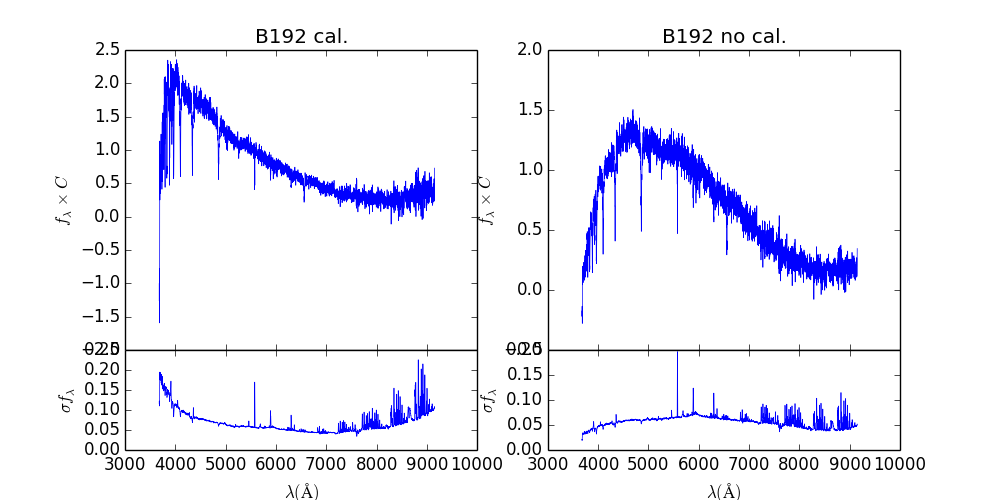
\includegraphics[width = 0.5 \textwidth]{figures/dfig_b192-g242_020.png}
\caption{A mock spectrum for a star cluster with the fiducial
parameters $10^5 M_\odot$ total stellar mass, an age of 9 Gyr, solar
metallicity, and $A_V=0.5$ mag. \label{fig:mock_data}}
\end{figure}


\begin{figure*}[h!]
%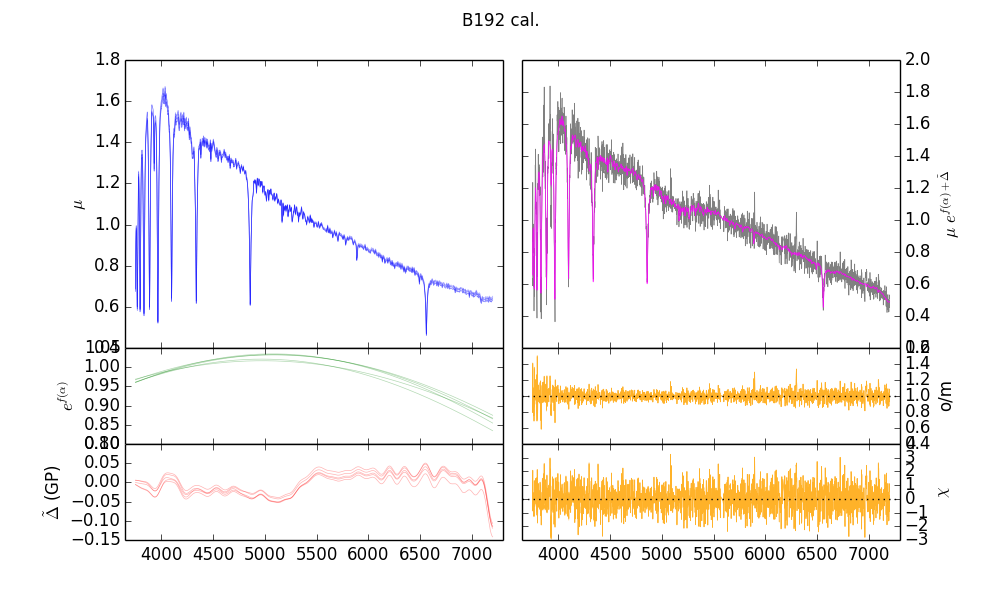
\includegraphics[width=\textwidth]{figures/sfig_b192-g242_225_cal.png}
\caption{Results of inference from a mock spectrum and a single photometric data point where the spectrophotometric calibration is assumed to be perfectly known.
Top Left: The mock observed spectrum ({\it black}) is shown as well as
YY model spectra constructed from draws from the posterior PDFs of the
model parameters, including calibration parameters {\it green}.
Bottom Left: In this case the true calibration vector ({\it black}) is a constant.
Posterior samples of the inferred calibration vector ({\it green}) include both
the polynomial and the Gaussian Process mean prediction (Equation
\ref{eq:calibration}).
Top Right: Samples of the posterior prediction for the
\emph{intrinsic} spectrum ({\it green}) as well as for the photometry
({\it magenta}).  The true mock photometry is also shown ({\it
black}).
Bottom Right: Marginalized posterior PDFs for several of the physical
parameters of interest.  The input mock parameters are shown as
vertical lines.
\label{fig:speconly_ideal}}
\end{figure*}


\begin{figure*}[h!]
%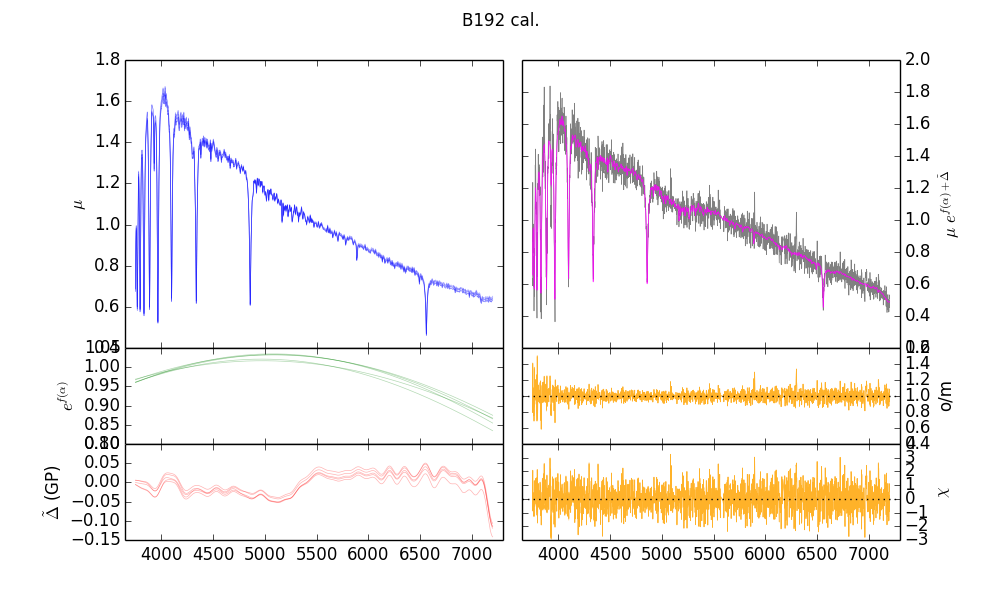
\includegraphics[width=\textwidth]{figures/sfig_b192-g242_225_cal.png}
\caption{Results of inference from a \emph{perfectly calibrated} mock
  spectrum and a single photometric data point.
Top Left: The mock observed spectrum ({\it black}) is shown as well as
YY model spectra constructed from draws from the posterior PDFs of the
model parameters, including calibration parameters {\it green}.
Bottom Left: In this case the true calibration vector ({\it black}) is a constant.
Posterior samples of the inferred calibration vector ({\it green}) include both
the polynomial and the Gaussian Process mean prediction (Equation
\ref{eq:calibration}).
Top Right: Samples of the posterior prediction for the
\emph{intrinsic} spectrum ({\it green}) as well as for the photometry
({\it magenta}).  The true mock photometry is also shown ({\it
black}).
Bottom Right: Marginalized posterior PDFs for several of the physical
parameters of interest.  The input mock parameters are shown as
vertical lines.
\label{fig:speconly_calibrated}}
\end{figure*}

\begin{figure*}[h!]
%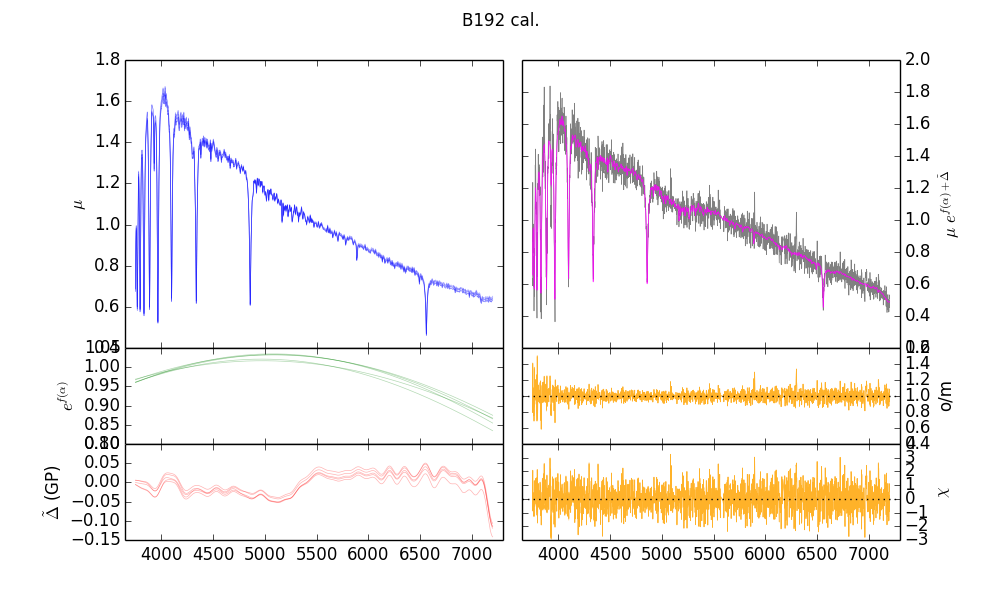
\includegraphics[width=\textwidth]{figures/sfig_b192-g242_225_cal.png}
\caption{Results of inference from an \emph{uncalibrated} mock
  spectrum and a single photometric data point.  Panels and colors are
  as in Figure \ref{fig:speconly_calibrated}.  In this case the
  observed spectrum is in arbitrary units and the true
  calibration vector is not a constant with wavelength.
\label{fig:speconly_uncalibrated}}
\end{figure*}

\begin{figure*}[h!]
%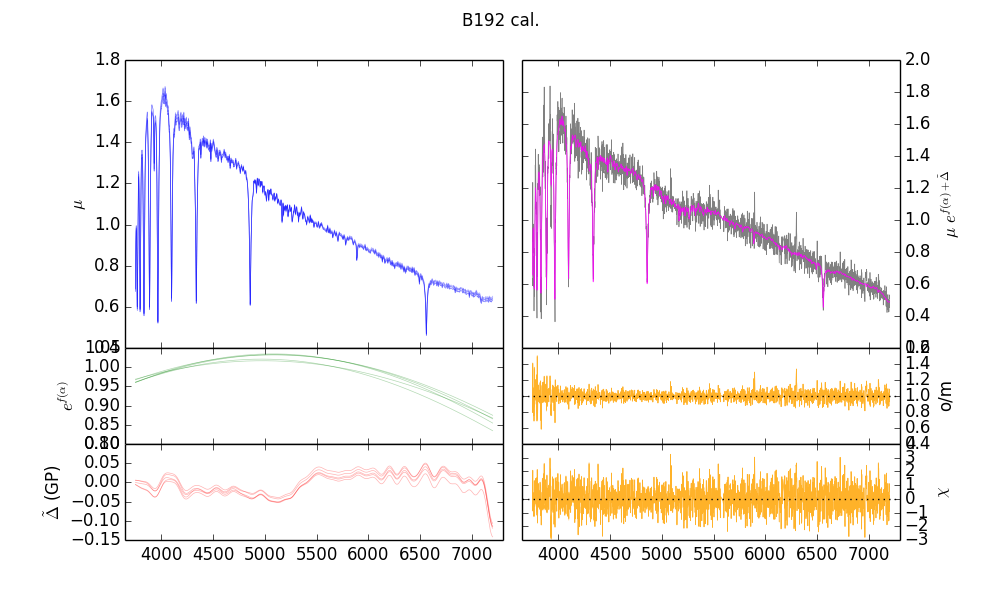
\includegraphics[width=\textwidth]{figures/sfig_b192-g242_225_cal.png}
\caption{Results of inference from the photometric data only.
Top: The intrinsic spectrum. Samples of the posterior prediction
for the \emph{intrinsic} spectrum ({\it green}) and the
photometry ({\it magenta}).  The mock photometry is also shown
({\it black}).
Right: Marginalized posterior PDFs for several of the physical
parameters of interest.  The input mock parameters are shown as
vertical lines.
\label{fig:photonly}}
\end{figure*}

\begin{figure*}[h!]
%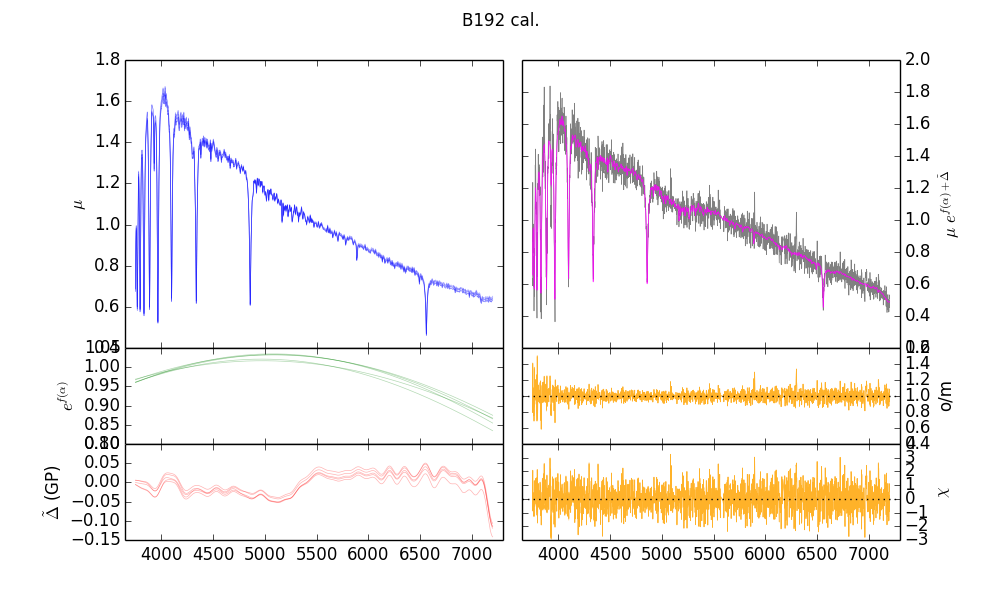
\includegraphics[width=\textwidth]{figures/sfig_b192-g242_225_cal.png}
\caption{Results of inference from the combination of
  \emph{uncalibrated} spectroscopy and all the photometric data
  points.  Panels and colors are as in Figure \ref{fig:speconly_calibrated}.
\label{fig:speconly_calibrated}}
\end{figure*}


\begin{figure*}[h!]
%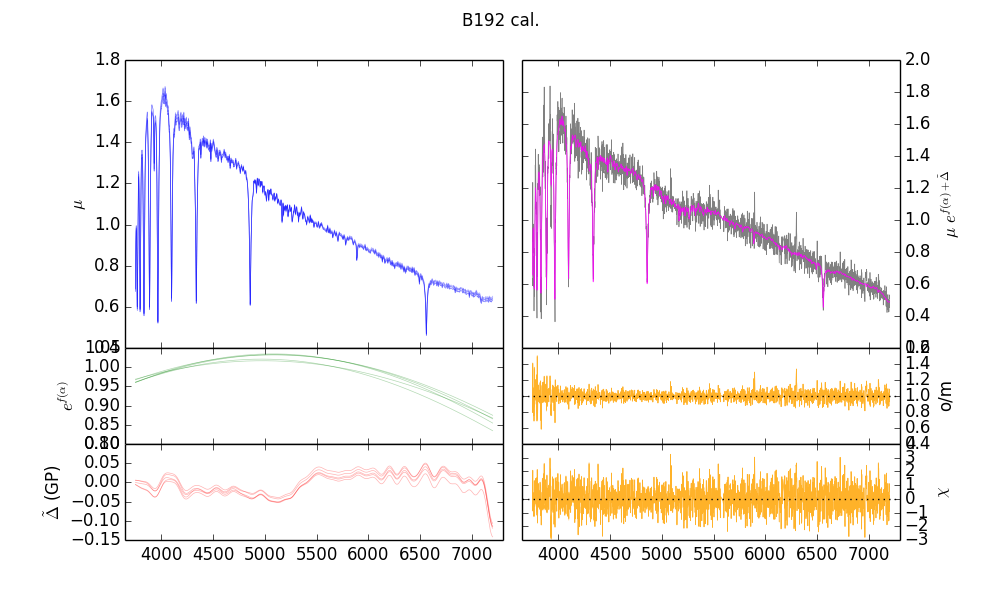
\includegraphics[width=\textwidth]{figures/sfig_b192-g242_225_cal.png}
\caption{Joint posterior PDFs for several physical parameters. The
  posteriors obtained from photometry only is in {\it red}, from
  \emph{uncalibrated} spectroscopy and a single photometric point in {\it blue}, and from
  the photometry and spectroscopy combined in {\it magenta}.
\label{fig:combined_posterior}}
\end{figure*}


\begin{figure*}[h!]
%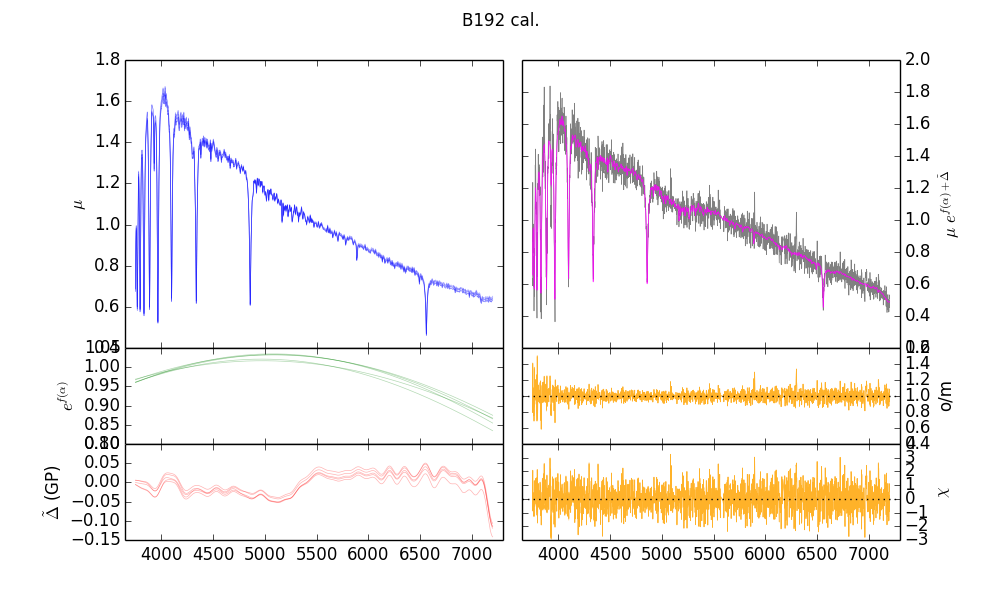
\includegraphics[width=\textwidth]{figures/sfig_b192-g242_225_cal.png}
\caption{Posterior PDFs obtained from multiple noise realizations of the
  mock photometry and uncalibrated spectra, for a single set of
  parameters.  The input mock parameters are shown as a 
  vertical line, medians of the posterior CDF for each realization are
  shown as dotted lines.
\label{fig:noise_realizations}}
\end{figure*}


\begin{figure*}[h!]
%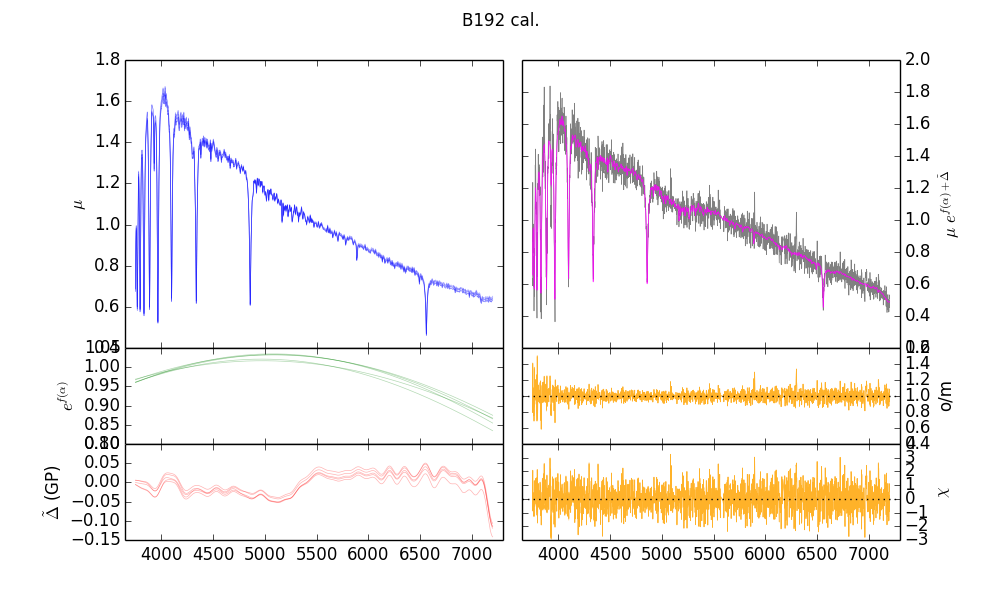
\includegraphics[width=\textwidth]{figures/sfig_b192-g242_225_cal.png}
\caption{Posterior PDFs obtained from mock spectra and photometry
  created with  a variety of mock physical parameters, as a function
  of those parameters.
\label{fig:mock_parameter_space}}
\end{figure*}


\end{document}
